\Chapter{Tervezés}

\Section{Grafikus felhasználói felület (GUI) - megjelenés, funkció}

Ebben a fejezetben, ahogy kezd a program kialakulni, úgy lehetséges a leírt elképzelések változása is. Az elképzelt program és a végeredmény összehasonlítása valószínűleg a következő fejezet végén lesz elhelyezve.

Az alkalmazás három (vagy kettő) fő menüpontből fog állni, a főmenü, jegyzetek menü és keresés menü. Vannak olyan elemek, amik minden menüpontban látszanak és használhatóak, ezek leírása következik:

\begin{figure}[h]
	\centering
	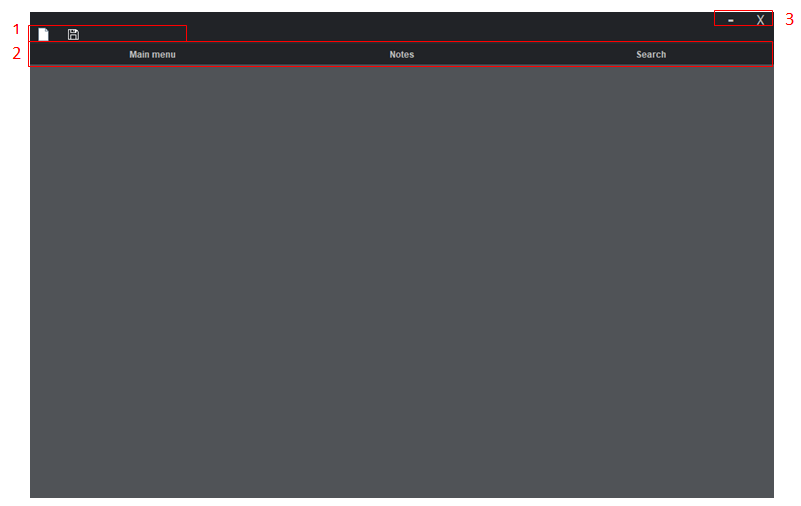
\includegraphics[scale=0.7]{images/menu_1.png}
	\caption{Program 'körvonala', alapja, a felület amire a többi menü épül.}
	\label{fig:main_foundation}
\end{figure}

\noindent \textbf{1.} Gombok helye. Egyelőre fájl megnyitása és mentése gomb található itt, viszont nem funkcionálisak még. Ha további gombok hozzáadása szükséges lesz, akkor azok is itt fognak elhelyezkedni, feltéve ha mind a három menüpontban használhatóak.
\vspace{5pt} \\Fájl mentése: elmenti a fájlokat az adatbázisba. Gyorsbillentyű: Ctrl + S. A program jelenlegi tervek szerint nem menti el az adatokat automatikusan, ennek megváltozása a későbbiekben lehetséges.
\vspace{5pt} \\Fájl megnyitása: ha esetleg egy másik számítógépről szeretnénk jegyzeteket betölteni, akkor ez a menüpont tud majd lehetőséget nyújtani ennek kivitelezésére.\vspace{5pt}

\noindent \textbf{2.} Három fő menüpont helye, ezekre kattintva váltogathatunk majd köztük.
\vspace{5pt} \\ \textbf{3.} Bezárás és tálcáz gombok, funkcióik egyértelműek.
\vspace{5pt} \\A bal felső sarokba szeretnék majd még egy logo-t rakni. Az alkalmazás bárhová elhelyezhető a képernyőn (tehát lehet húzgálni) viszont fix méretű.
\vspace{5pt} \\Belépéskor ez a kép fogadja a felhasználót, egyik menüpontban sincs benne ilyenkor.

\subsection{Főmenü}

\begin{figure}[h]
	\centering
	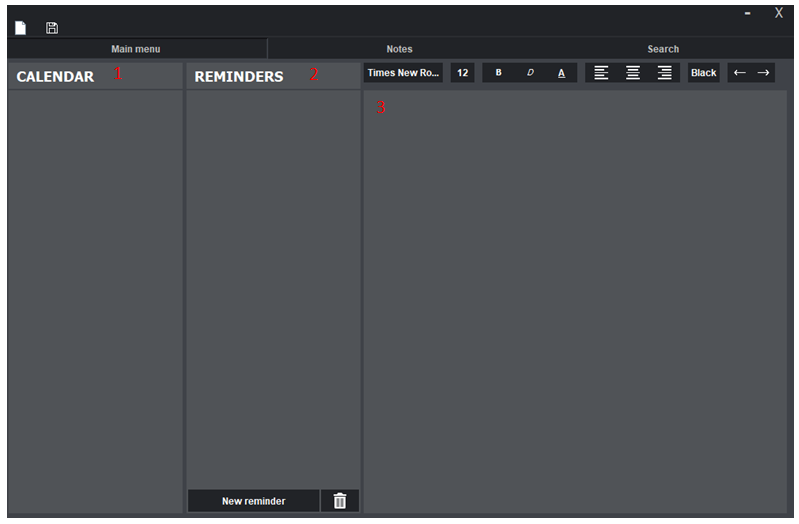
\includegraphics[scale=0.7]{images/menu_2.png}
	\caption{Főmenü, naptár-emlékeztető egyben.}
	\label{fig:menu_main}
\end{figure}

\noindent Ez az egész menü nem biztos, hogy a kész alkalmazásban szerepelni fog, időtől függ és attól, hogy egy használható naptár-emlékeztető rendszert sikerül-e implementálnom. Ha sikerül, akkor:
\vspace{5pt} \\ \textbf{1.} Itt lesz a naptár látható, időben előre, hátra lehet benne haladni. Napokat ki lehet kattintással jelölni.
\vspace{5pt} \\ \textbf{2.} A naptárban kijelölt nap emlékeztetőinek listája található itt. A kijelölt naphoz lehet emlékeztetőt létrehozni valamint emlékeztetőt törölni. A törlés az éppen kijelölt emlékeztetőt törli. 
\vspace{5pt} \\ \textbf{3.} Jelenleg egy szövegszerkesztő menü (erről a következő menüben bővebben) található itt, hogy az éppen kijelölt emlékeztető tartalmát lehessen szerkeszteni, de ez valószínűleg változni fog. Ennek mérete a felére fog csökkenni és a szövegmező alá fog kerülni egy menü, amivel a kijelölt emlékeztető beállításait lehet majd szerkeszteni (pl, hogy hány nappal, perccel emlékeztessen a megadott nap előtt, stb..), valamint az emlékeztető létrehozását lebonyolító menü helye is itt lesz.

\subsection{Jegyzetek menü}

\begin{figure}[h]
	\centering
	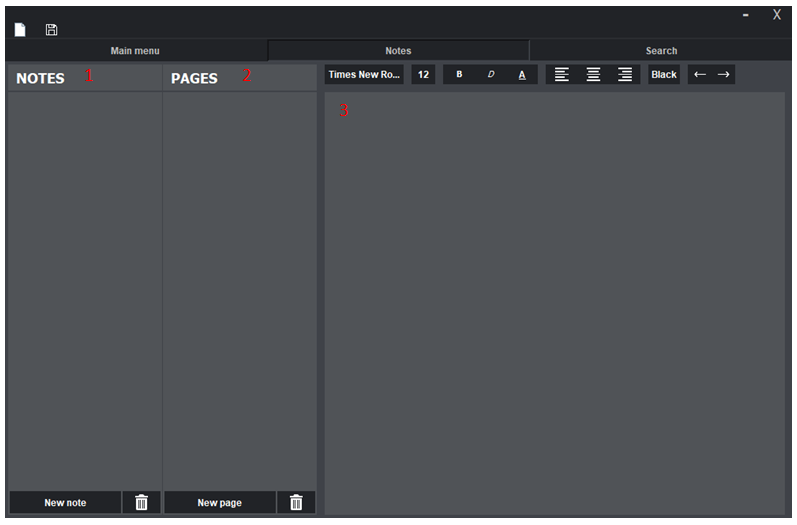
\includegraphics[scale=0.7]{images/menu_3.png}
	\caption{Jegyzetek menü}
	\label{fig:menu_notes}
\end{figure}

\vspace{5pt} \noindent \textbf{1.} Jegyzetek listája itt található. Egy ’note’ tulajdonképpen egy kategóriát jelent (pl jelszavak). Létrehozni és törölni jegyzeteket a lista alján található gombokkal lehet. Ha betelne a jegyzetek listája, akkor egy görgő segítségével lehet köztük navigálni. Létrehozni és törölni jegyzeteket a lista alján található gombokkal lehetséges. A gombok a kijelölt jegyzeteket szerkesztik.
\vspace{5pt} \\ \textbf{2.} Ha nincs jegyzet kiválasztva, akkor a lista alapvetően üres. Az éppen kijelölt (rákattintott) jegyzet oldalai (pages) található itt. Egy jegyzethez több oldal is létrehozható, de egy oldal csak egy jegyzethez tartozhat (feltéve ha nem másoltuk be egy másik jegyzetbe ugyan azt a szöveget és adtunk a lapunknak hasonló címet). Ha betelne az oldalak listája, akkor egy görgő segítségével lehet köztük navigálni. Létrehozni és törölni oldalakat a lista alján található gombokkal lehetséges. A gombok a kijelölt oldalakat szerkesztik.
\vspace{5pt} \\ \textbf{3.} Szövegszerkesztő, az éppen kijelölt oldal tartalma látható és szerkeszthető itt. Ha nincs oldal kijelölve, akkor nem használható a szerkesztő. Szerkesztési lehetőségek a következőek: betűstílus, betűméret, dőlt, vastag és aláhúzott szöveg, balra, középre és jobbra igazítás, szöveg szín megadása, vissza és előre (ha vissza meg lett nyomva).

\subsection{Kereső menü}

\begin{figure}[h]
	\centering
	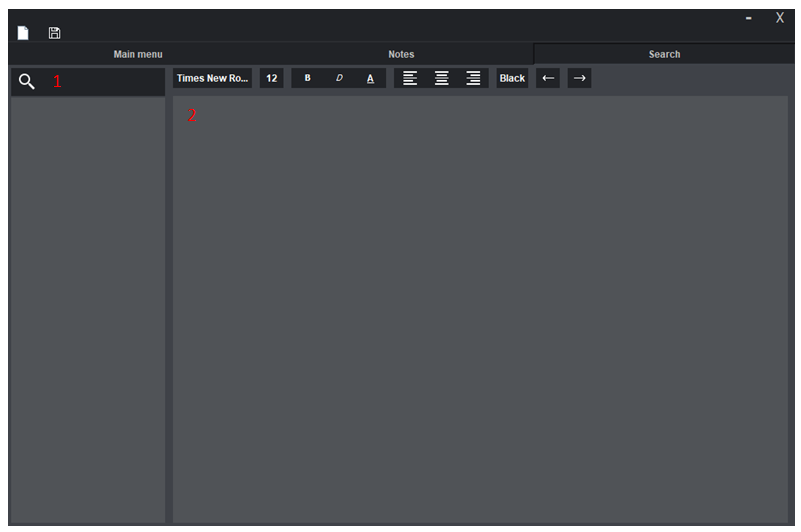
\includegraphics[scale=0.7]{images/menu_4.png}
	\caption{Kereső menü}
	\label{fig:menu_search}
\end{figure}

\vspace{5pt} \noindent \textbf{1.} Kereső sáv. Nem case-sensitive, tehát nem tesz kis- és nagybetű között különbséget. Beírt szövegre a nagyító gombra való kattintással tudunk rákeresni. Jegyzet- és oldalnevek között és ezek tartalma között is keres. (?)Hibásan begépelt szövegre is kiad valamilyen találatot.
\vspace{5pt} \\ \textbf{2.} Az előző fázisban bemutatott szövegszerkesztő. Ennek funkciója itt kérdéses, lehet, hogy nem is lesz itt, hanem egy keresési találtara való kattintás után a program vissza fog dobni a megfelelő menüpontba. De lehet, hogy itt marad és akkor a keresési találatok szövege lesz itt szerkeszthető (feltéve ha egy lap találtara kattintunk, nem egy jegyzetre).




\newpage
Ez a fejezet mutatja be a megvalósítás lépéseit.
Itt lehet az esetlegesen előforduló technikai nehézségeket említeni.
Be lehet már mutatni a program elkészült részeit.

Meg lehet mutatni az elkészített programkód érdekesebb részeit.
(Az érdekesebb részek bemutatására kellene szorítkozni.
Többségében a szöveges leírásnak kellene benne lennie.
Abból lehet kiindulni, hogy a forráskód a dolgozathoz elérhető, azt nem kell magába a dolgozatba bemásolni, elegendő csak behivatkozni.)

A dolgozatban szereplő forráskódrészletekhez külön vannak programnyelvenként stílusok.
Python esetében például így néz ki egy formázott kódrészlet.
\begin{python}
import sys

if __name__ == '__main__':
    pass
\end{python}

A stílusfájlok a \texttt{styles} jegyzékben találhatók.
A stílusok között szerepel még C++, Java és Rust stílusfájl.
Ezek használatához a \texttt{dolgozat.tex} fájl elején \texttt{usepackage} paranccsal hozzá kell adni a stílust, majd a stílusfájl nevével megegyező környezetet lehet használni.
További példaként C++ forráskód esetében ez így szerepel.
\begin{cpp}
#include <iostream>

class Sample : public Object
{
    // An empty class definition
}
\end{cpp}
Stílusfájlokból elegendő csak annyit meghagyni, amennyire a dolgozatban szükség van.
Más, C szintaktikájú nyelvekhez (mint például a JavaScript és C\#) a Java vagy C++ stílusfájlok átszerkesztésére van szükség.
(Elegendő lehet csak a fájlnevet átírni, és a fájlban a környezet nevét.)

Nyers adatok, parancssori kimenetek megjelenítéséhez a \texttt{verbatim} környezetet lehet használni.
\begin{verbatim}
$ some commands with arguments
1 2 3 4 5
$ _
\end{verbatim}

A kutatás jellegű témáknál ez a fejezet gyakorlatilag kimaradhat.
Helyette inkább a fő vizsgálati módszerek, kutatási irányok kaphatnak külön-külön fejezeteket.
